\subsection{20 августа. пер. Уллукёль Восточный (1А*)}
\textit{Метеоусловия: утром, днём ясно, вечером~--- переменная облачность, тепло.}

\begin{figure}[h!]
	\centering
	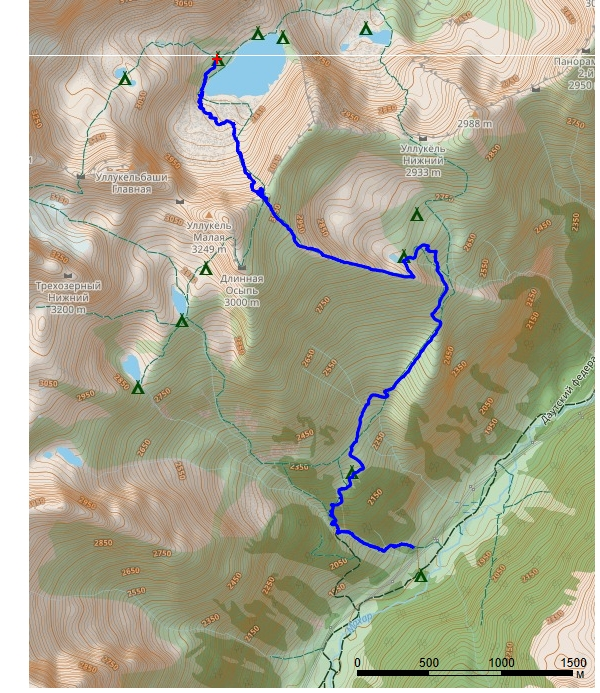
\includegraphics[angle=0, width=0.7\linewidth]{../pics/mini_maps/20}
	\label{fig:mini_20}
\end{figure}

Подъём дежурных в 04:30, общий подъём в 05:00. Выход группы в 07:30 (рис.~\ref{fig:20aug1.jpg}).

\begin{figure}[h!]
	\centering
	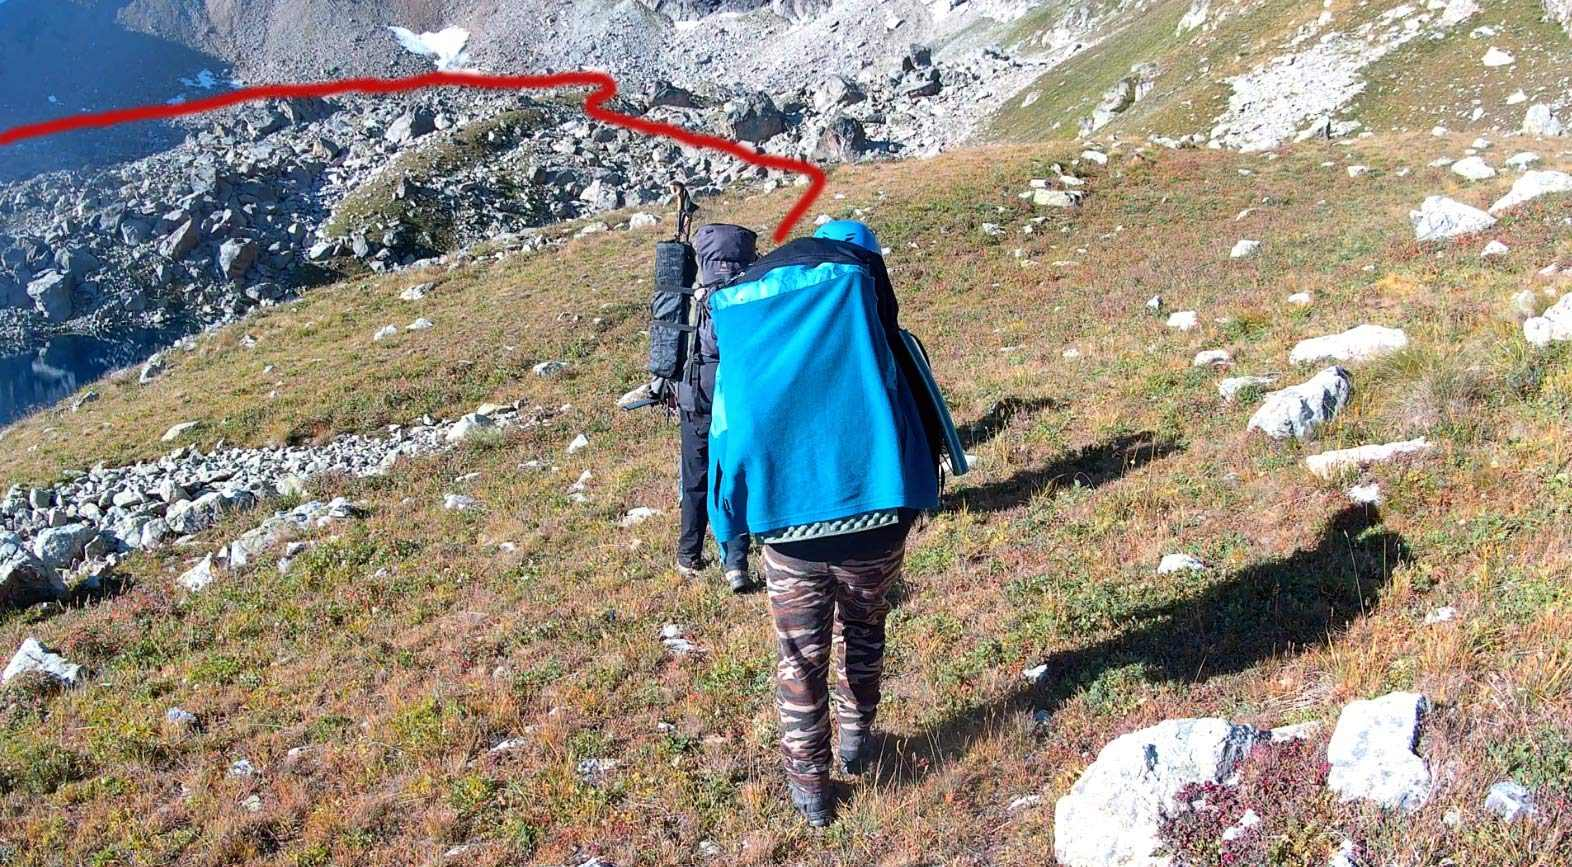
\includegraphics[width=0.7\linewidth]{../pics/20aug1.jpg}
	\caption{Подход под перевал от м.н.}
	\label{fig:20aug1.jpg}
\end{figure}


Начали движение по разведанному вчера маршруту по крупной осыпи в обход южной оконечности озера. Ночью у одной из участниц, Наташи Мироновой, случилось сильное желудочное расстройство, и после первого  привала --- собственно у начала участка с валунами --- у неё забрали рюкзак, и небольшой участок (ок. 15 мин. ЧХВ) Наташа прошла без рюкзака. Пока зам руководителя, Лёша Остапив, доносил Наташин рюкзак, а сама она принимала дополнительные лекарства, и мы дожидались улучшения, остальная часть группы фотографировалась на фоне озера на небольшом зелёном гребешке (рис.~\ref{fig:DSC_0907}). \alert{(Сюда или в 19-е поместить єту фотку: \ref{ullu_koel_lake_stones})} 
\begin{figure}[h!]
	\centering
	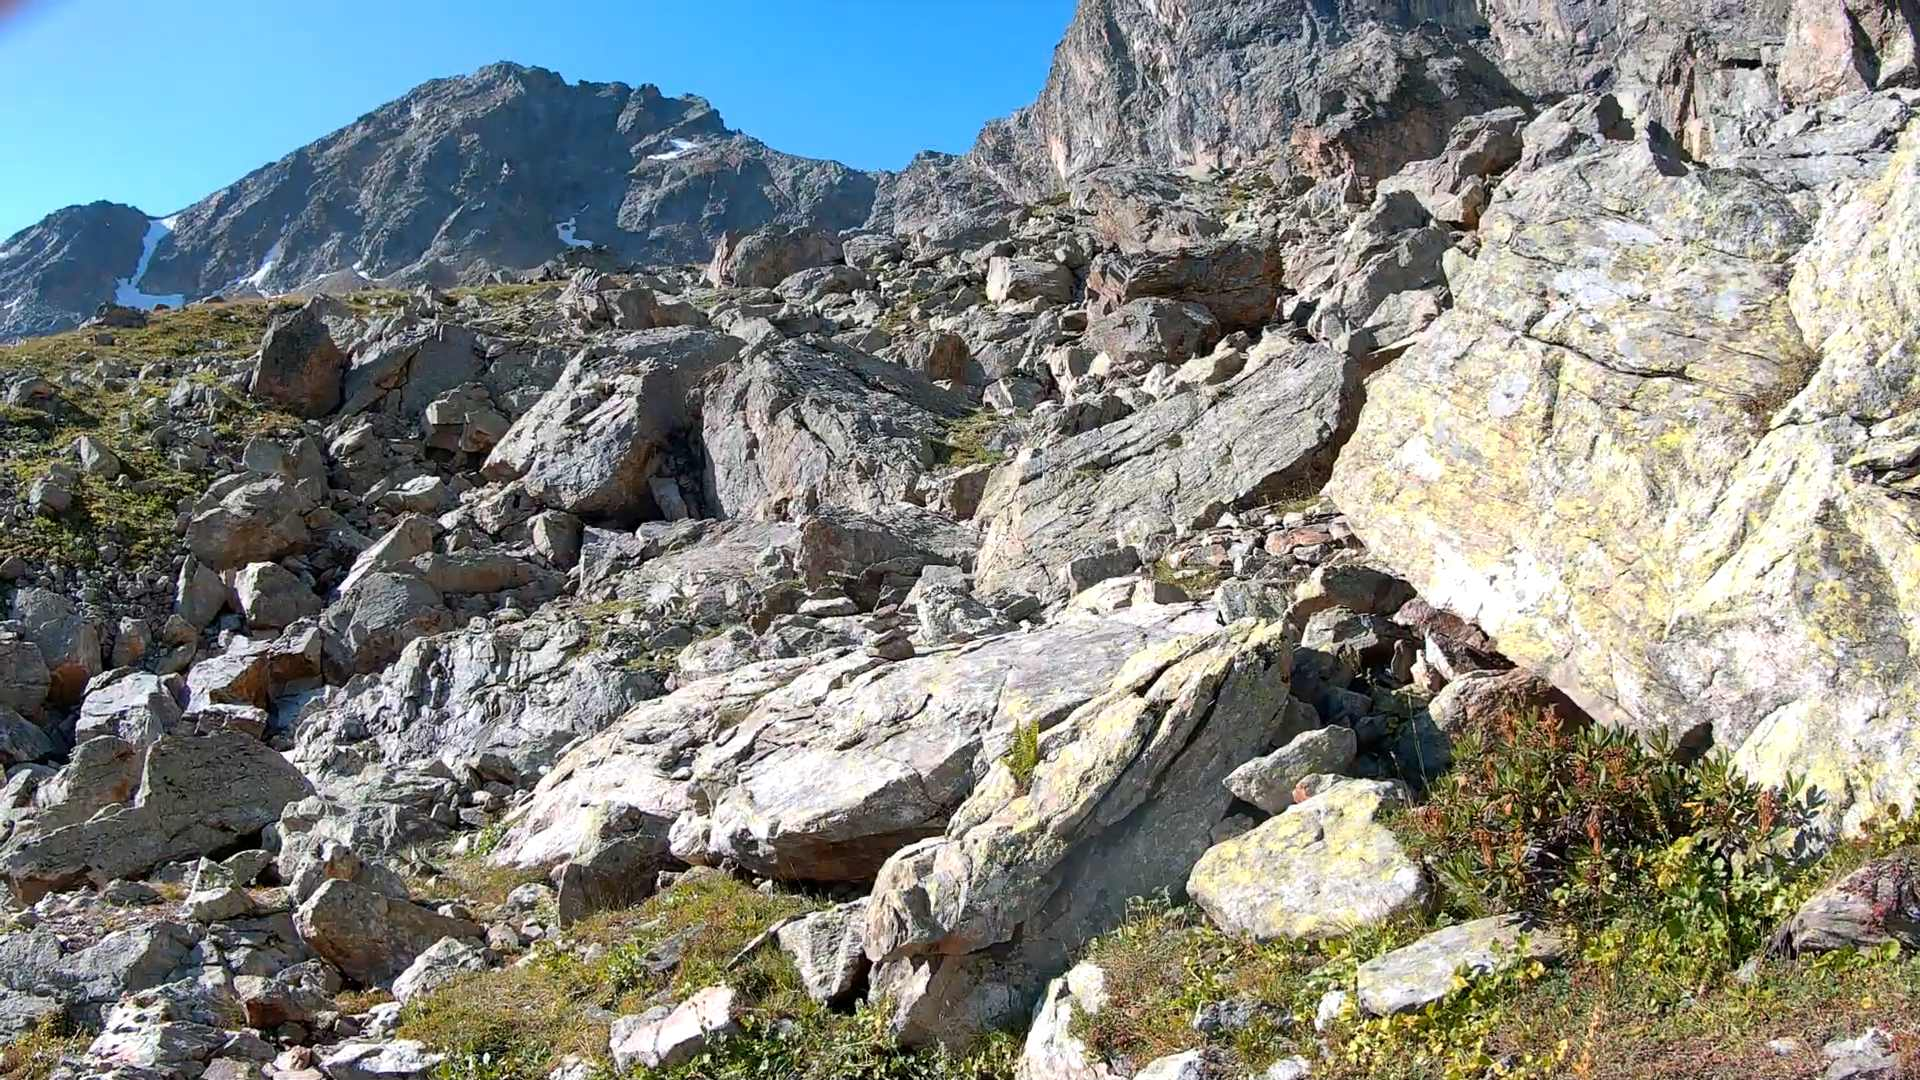
\includegraphics[width=0.7\linewidth]{../pics/ullu_koel_lake_stones.png}
	\caption{Прохождение участка с валунами у оз. Уллу-Кёль}
	\label{ullu_koel_lake_stones}
\end{figure}

 
 \begin{figure}[h!]
 	\centering
 	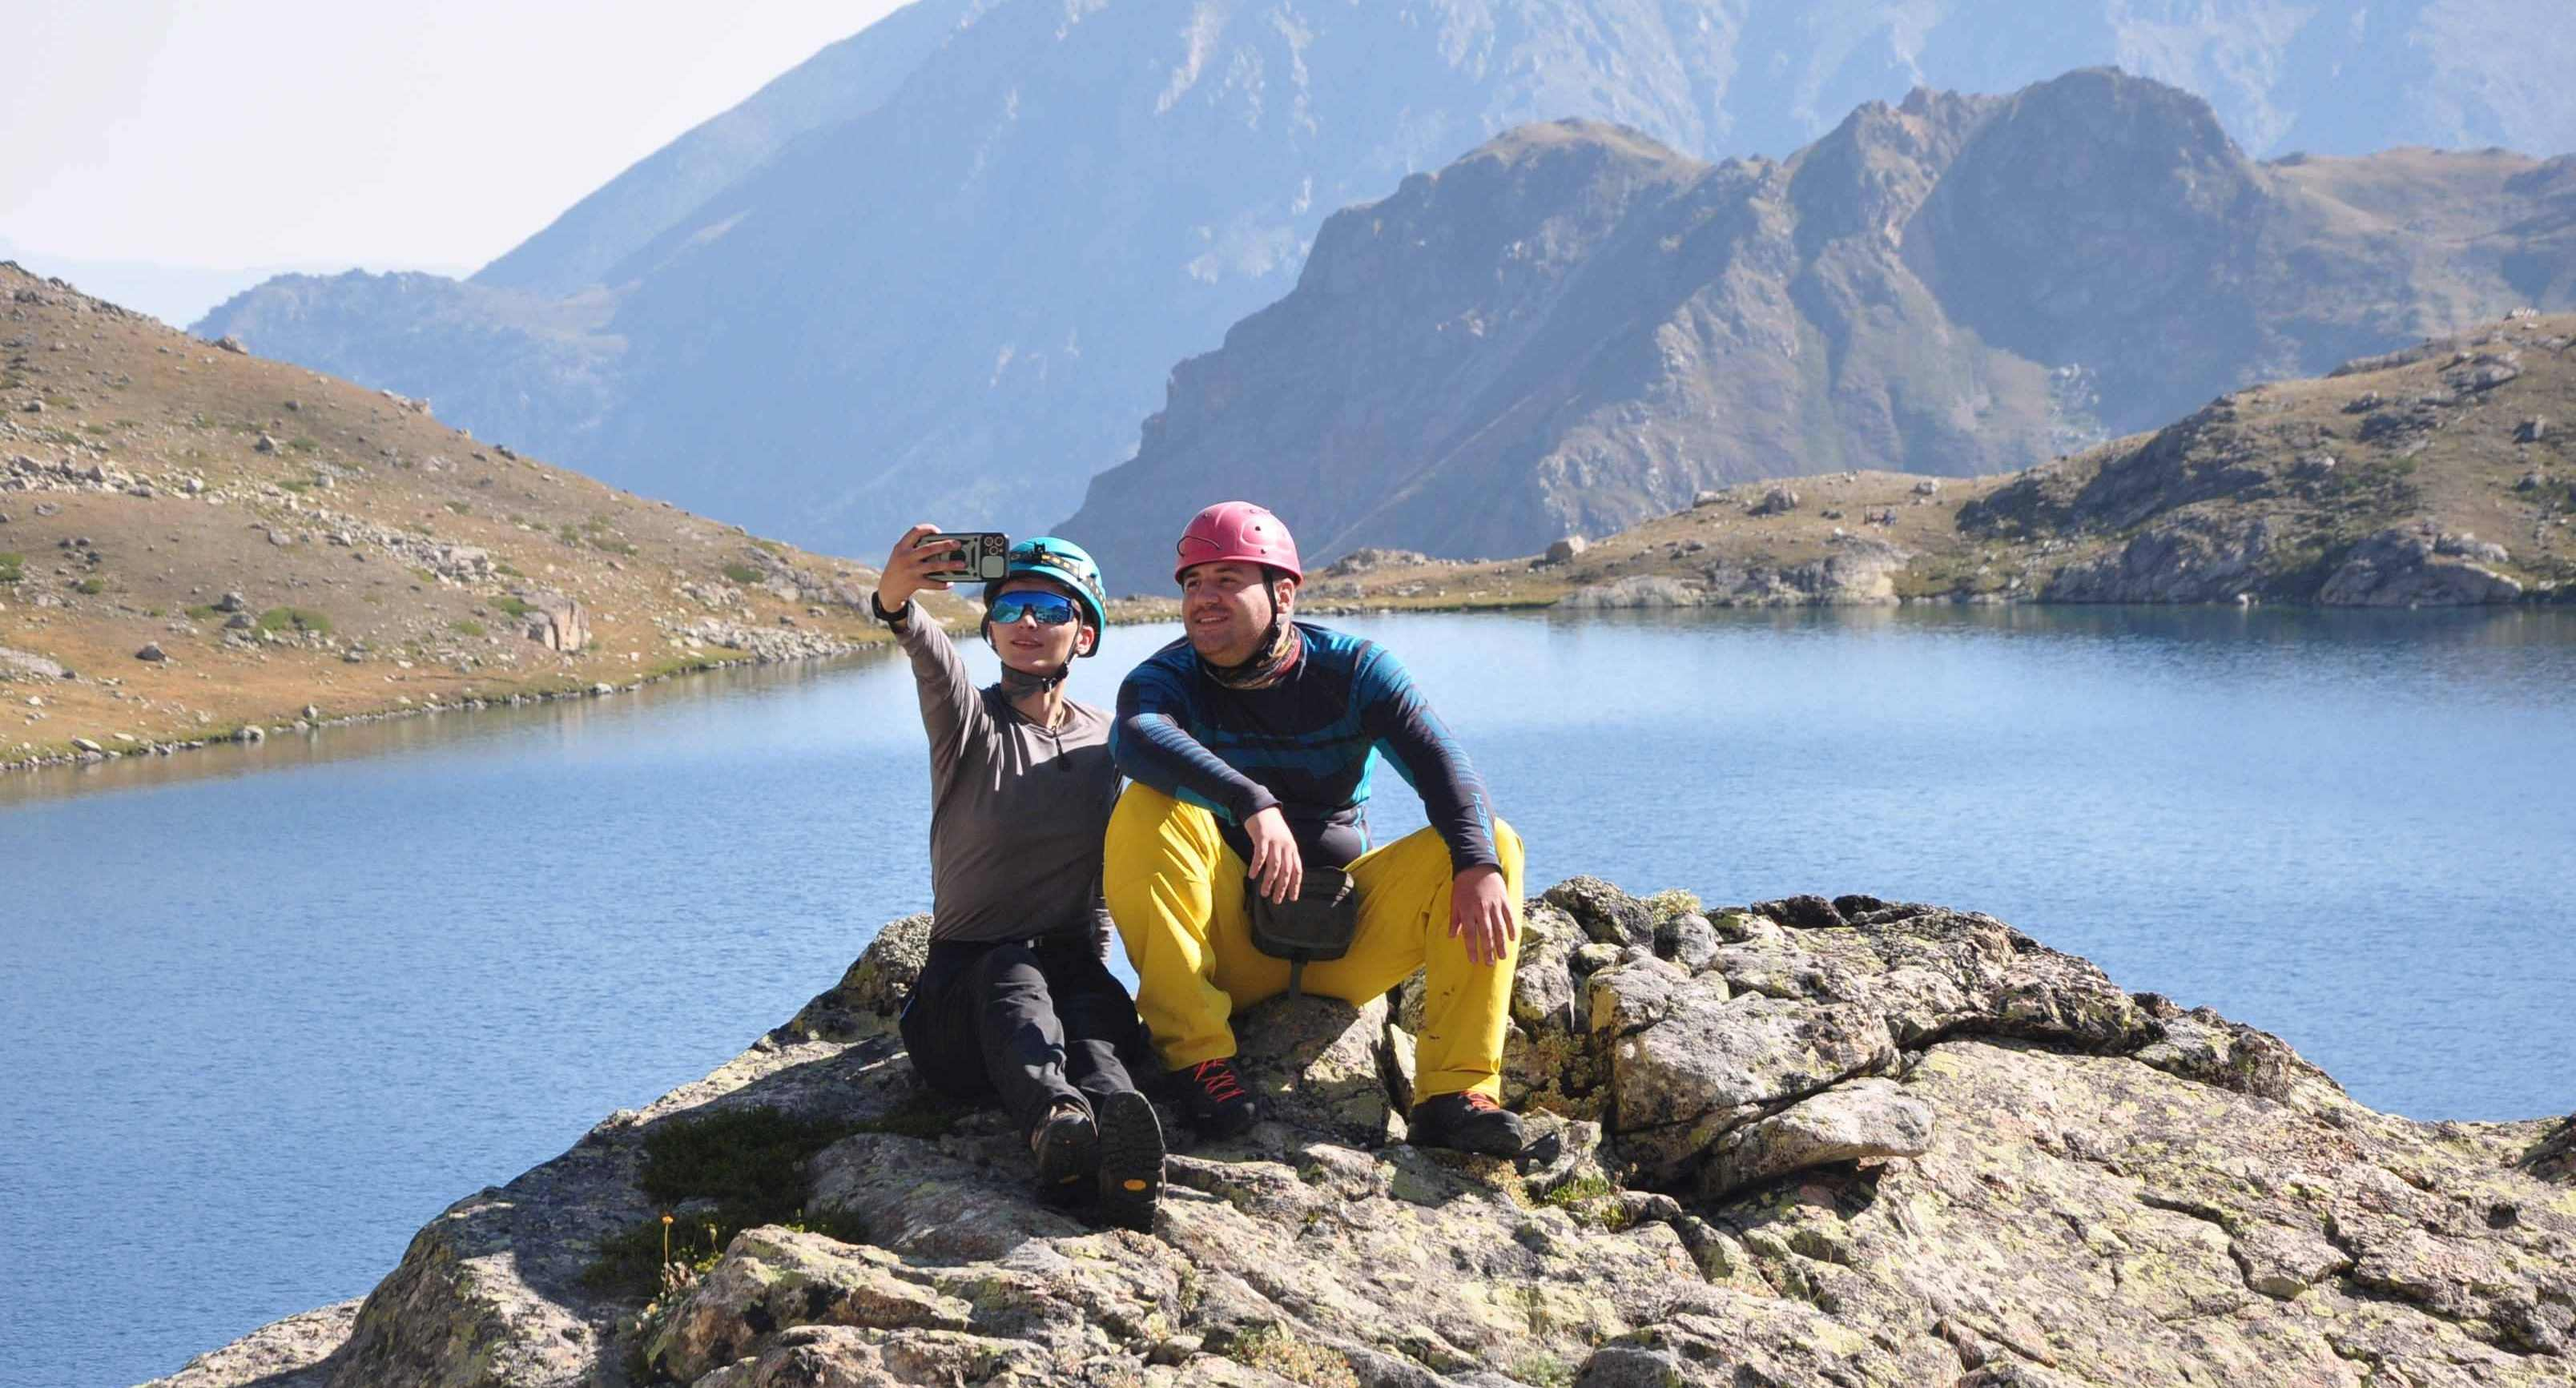
\includegraphics[width=0.7\linewidth]{../pics/DSC_0907}
 	\caption{Фоткаемся на фоне озера}
 	\label{fig:DSC_0907}
 \end{figure}
 

Далее двигались на юго-восток по моренному лабириту. На пути, на развилке между двумя гребнями, выбрали правый пхд. Конечной точкой лабиринта оказалась огромная каменная плита размером с подъёмный мост, перекинутая между гребнями, --- дальше путь хорошо просматривался. На этом участке пути Наташа шла уже со своим рюкзаком, но разргруженным до 10 кг. Таким образом группа добралась до другого зелёного гребешка, ведущего под перевальный взлёт \alert{(За сколько ходок?)} (рис.~\ref{fig:20aug2.jpg}), и в 9:40 вышла на среднюю осыпь перевального взлёта, прижимаясь к правому пхд борту кулуара. Осыпь была живой, требовала внимания при движении и контроля неопытных участников. \alert{(Фотка с прохождением моренного лабиринта точно есть --- надо вставить!)}

\begin{figure}[h!]
	\centering
	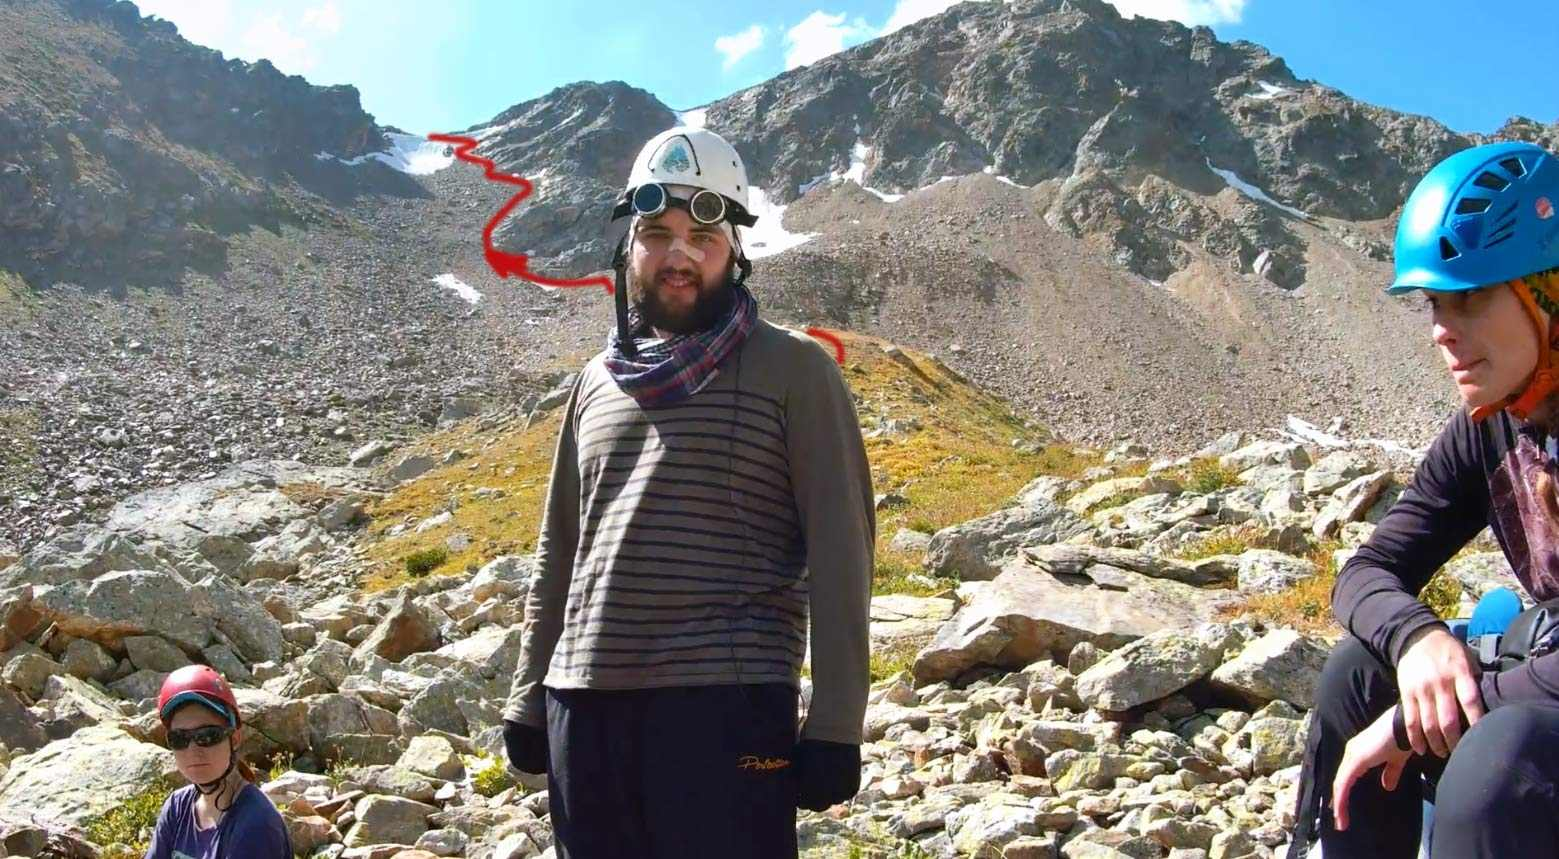
\includegraphics[width=0.7\linewidth]{../pics/20aug2.jpg}
	\caption{Маршрут движения по перевальному взлёту}
	\label{fig:20aug2.jpg}
\end{figure}

Снега на перевальном взлёте почти не было, поэтому руководитель принял решение двигаться не по середине кулуара, образующего взлёт, а по его правому борту, прижимаясь к скалам. Позже посередине кулуара удалось увидеть тропу, но руководитель решил сохранить намеченную траекторию, вдоль скал, из соображений камнеопасности. Осыпь на перевальном взлёте была живой, двигались плотной группой узким зигзагом (далее --- т.~н. <<галсами>>), не выходя на середину. На одном из участков попытались выбраться на скалы, но поняли, что это не имеет большого смысла, поскольку сил отбирает много, а потом всё равно приходится выходить на осыпь. В 12:25, за 6 ходок от старта, достигли полочки, на уровне которой начинается самая крутая часть перевального взлёта и снежник. Руководитель отдал команду группе надевать кошки, а сам с зам. руковода дошёл до середины кулуара, чтобы подобрать <<посаженный>> туда накануне коптер: хорошо, что он успел сообщить свои координаты! Поскольку ещё на старте похода выяснилось, что одна пара кошек осталась в Москве, руководитель отдал свои кошки участнику и пошёл замыкающим. В 13:16 группа надела кошки и выдвинулась косым траверсом влево пхд, целясь на выступающие из снега скалы и далее выше их --- на седловину. Снег был достаточно мягким, чтобы было возможно организовать ступени, однако лежал достаточно тонким слоем и к тому моменту подраскис. В связи с этим можно было либо идти на три такта, либо прижиматься к склону боком и ставить ногу на всю ступню. Вопрос о том, какой способ прохождения и, соответственно, организации ступеней лучше в данном случае, вызывал ожесточённую дискуссию между руководителем и замом, и к единому мнению прийти так и не удалось --- в итоге ступени имели <<компромиссную форму>>, заходя в снег под углом. На седловине снежного карниза не было, но присутствовал удобный снежный карман (рис.~\ref{fig:DSC_0946}). За 70 м тропёжки произвели две смены лидера.

\begin{figure}[h!]
	\centering
	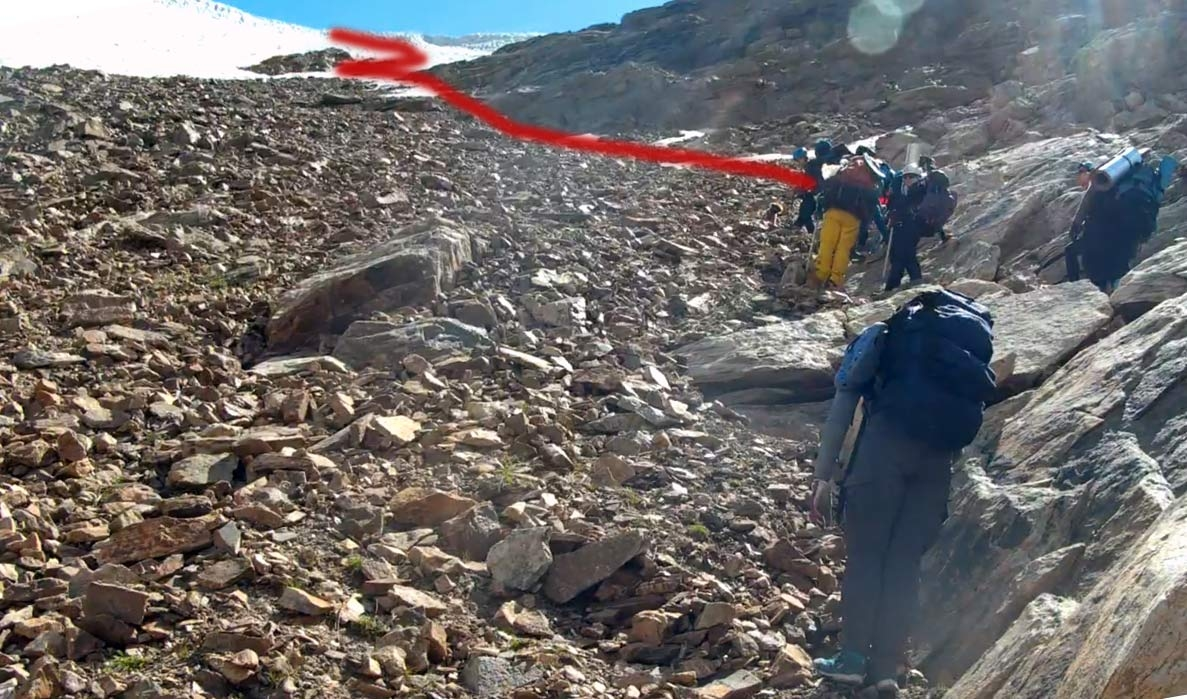
\includegraphics[width=0.7\linewidth]{../pics/20aug3.jpg}
	\caption{Движение по правому пхд борту кулуара}
	\label{fig:20aug3.jpg}
\end{figure}

\begin{figure}[h!]
	\centering
	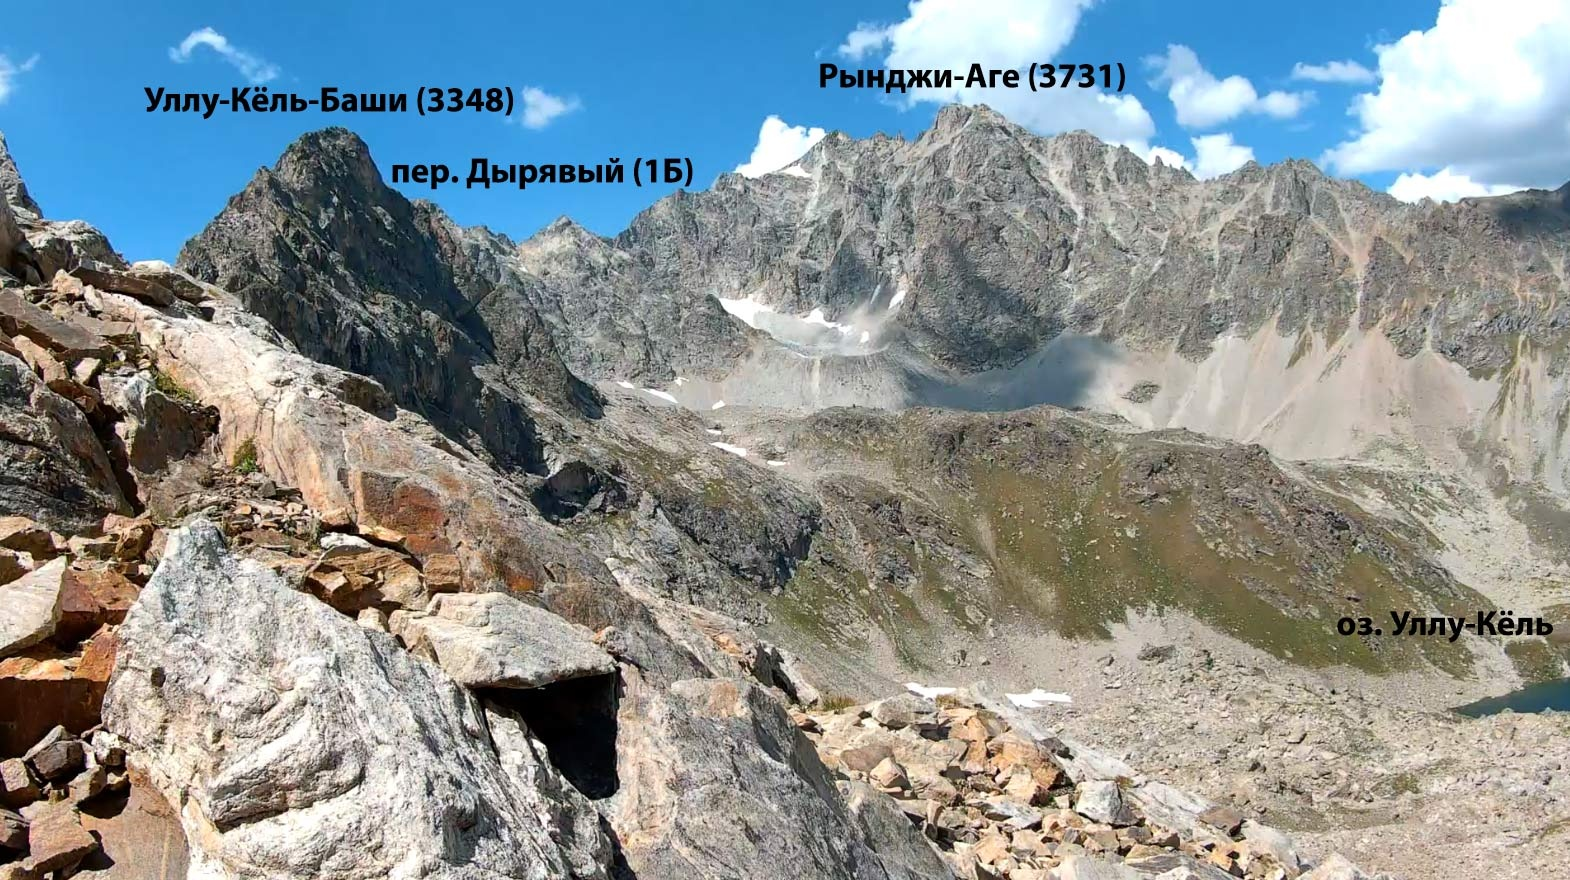
\includegraphics[width=0.7\linewidth]{../pics/20aug4.jpg}
	\caption{Вершины и перевалы цирка Уллу-Кёль}
	\label{fig:20aug4.jpg}
\end{figure}

Когда до снежного кармана (безопасной зоны) оставалось около 3 м по вертикали, лидер, Катя Тюрина, сорвалась. Причиной стала выскользнувшая из раскисшей ступени нога и то, что Катя взяла собаку в правую руку и хотела подсадить до выполаживания. Пролетев 50 метров по снежному склону крутизной 45\degree, Катя не успела окончательно зарубиться и остановилась только на осыпном склоне, перекувыркнушись через голову. Причинами тому были: а) дополнительное время на то, чтобы выпустить собаку и перехватить ледоруб; б) зацепившиеся друг за друга кошки. Замруководителя в этот момент шёл вторым; руководитель, как уже было сказано, последним. Сразу после падения голосовыми командами группа убедилась, что пострадавшая в сознании. Катя в течение минуты провела самостоятельный осмотр и убедилась в отсутствии сильных кровотечений, имея достаточный для того опыт (будучи медиком в группе). Руководитель отдал заму команду довести группу до безопасной зоны~--- снежного кармана, после чего спуститься к Кате. Последний человек покинул опасную зону спустя 7 минут после срыва, после чего руководитель и зам (Даша и Лёша) спустились к Кате, убедились, что она может идти самостоятельно, дали воду, еду и пуховку. Далее втроём поднимались к группе: Лёша нёс Катин рюкзак; Катя без рюкзака шла посередине (рис.~\ref{fig:DSC_0946}). Лидировали Даша и Лёша попеременно; вопрос о ступенях в этот момент вставал особенно остро --- разрешить его не удалось. 


\begin{figure}[h!]
	\centering
	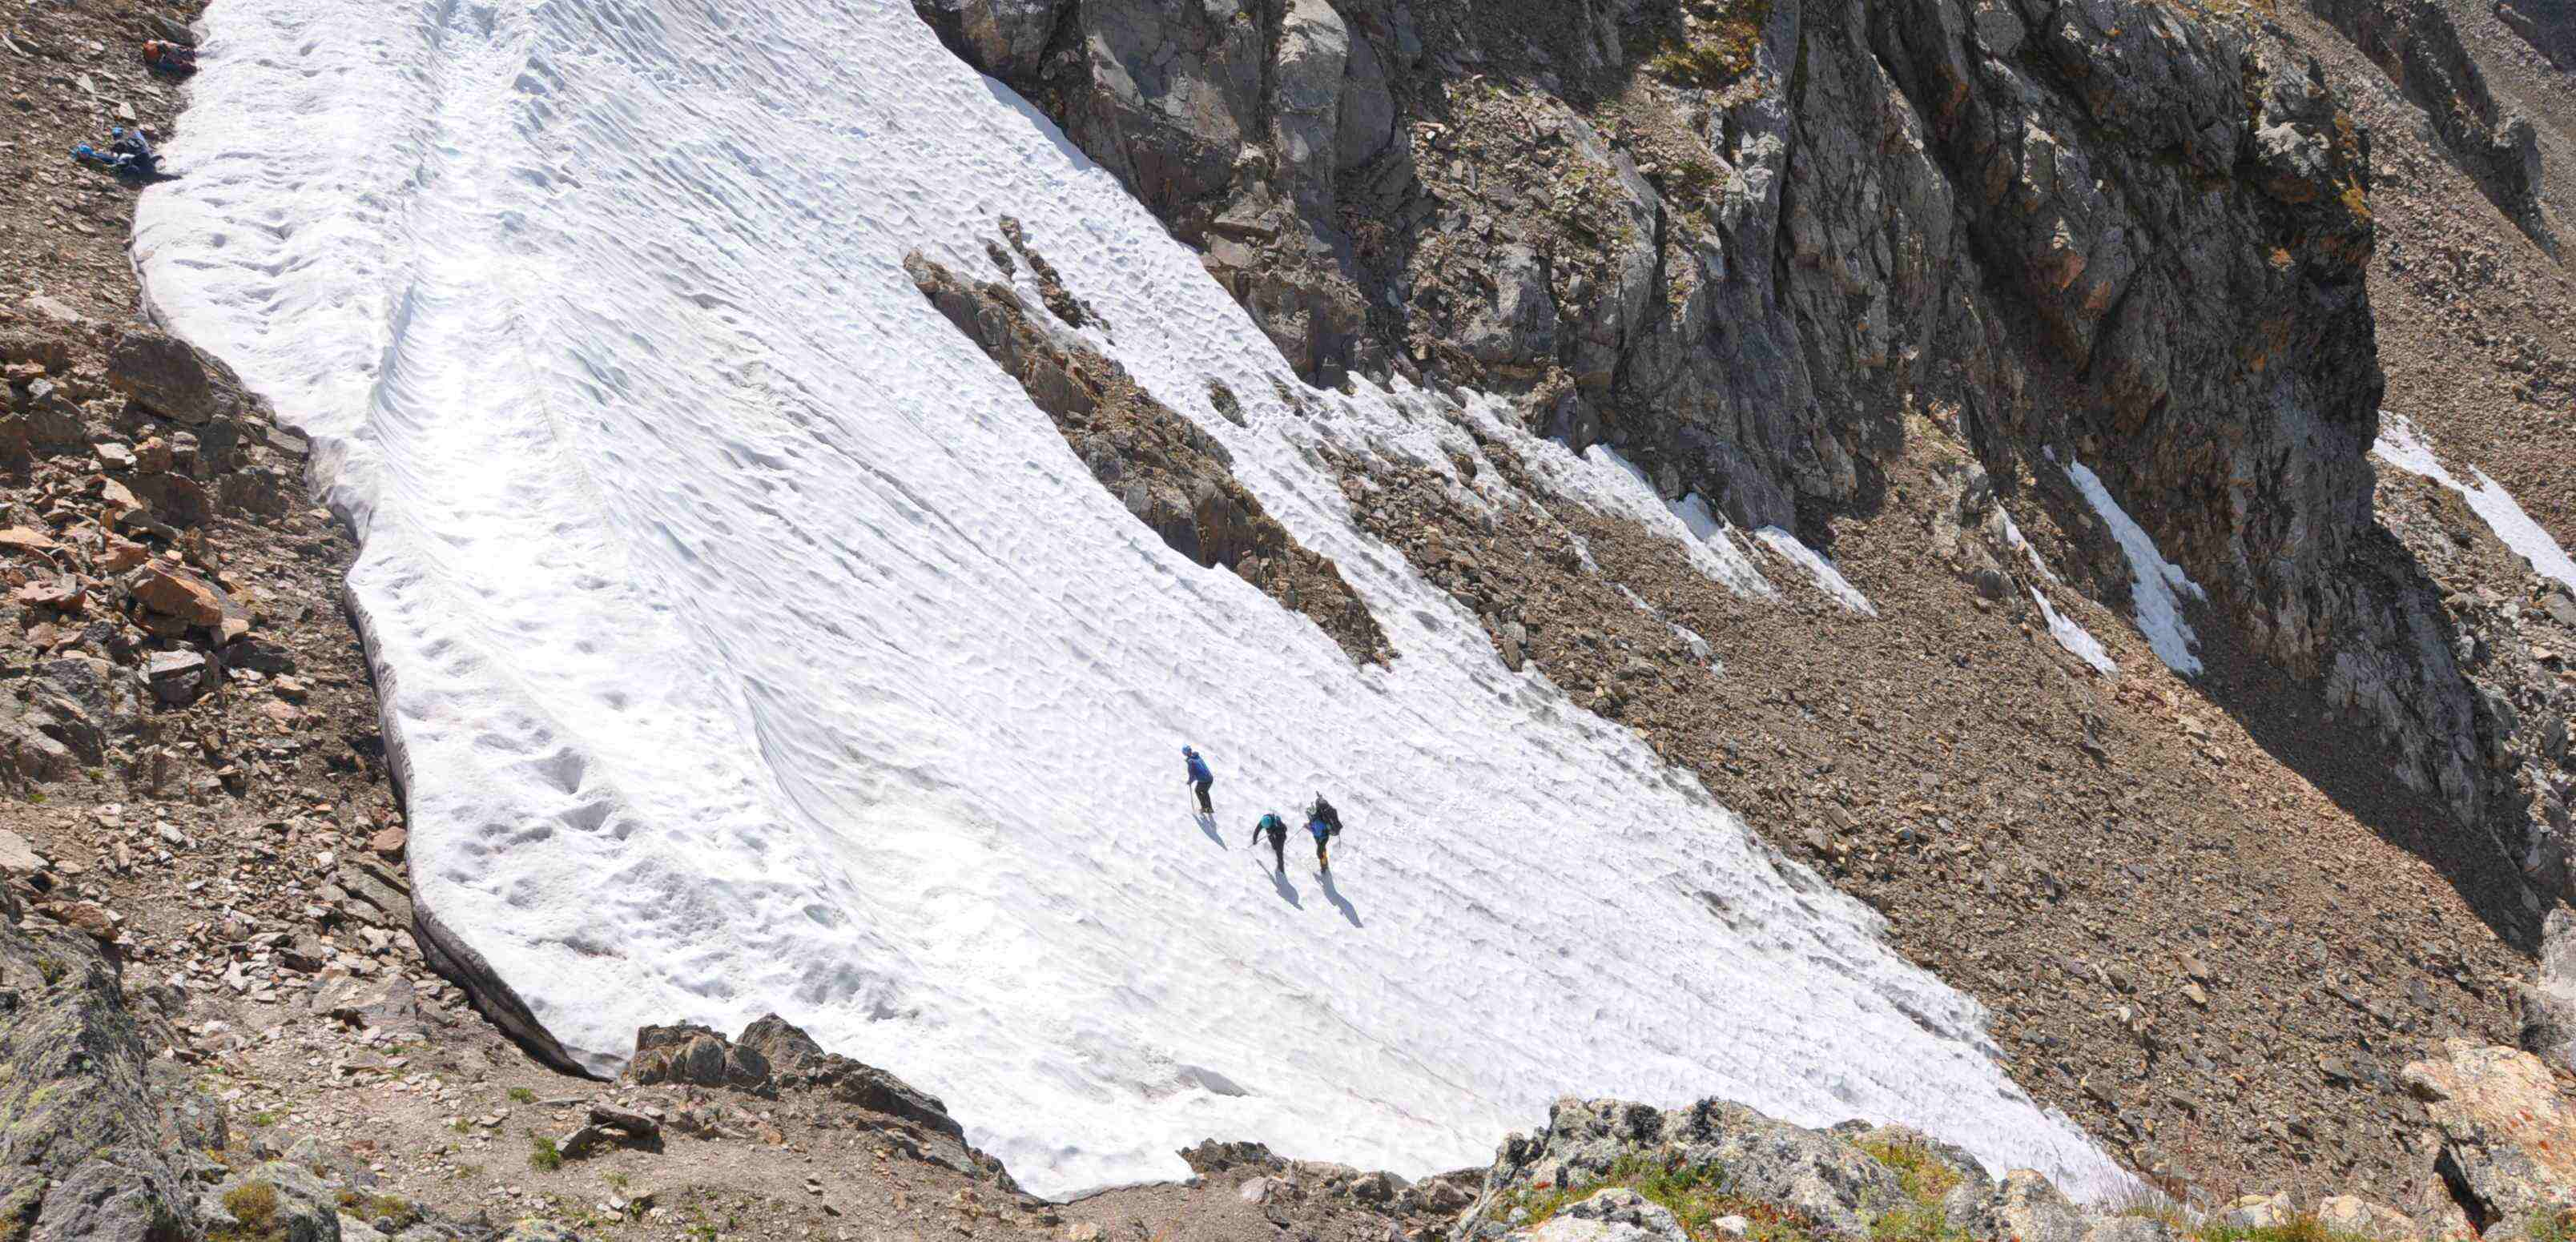
\includegraphics[width=0.7\linewidth]{../pics/DSC_0946.png}
	\caption{Маршрут движения группы по снежнику (красный), траектория срыва участника (синий), маршрут подъёма с сорвавшимся участником (чёрный)}
	\label{fig:DSC_0946}
\end{figure}


Вся группа собралась на седловине в 14:30, спустя 1 ч 05 мин с момента срыва. Сняли записку туристов т/к <<Шторм>>, г. Санкт-Петербург, от 09.08.2024.


\begin{figure}[h!]
	\centering
	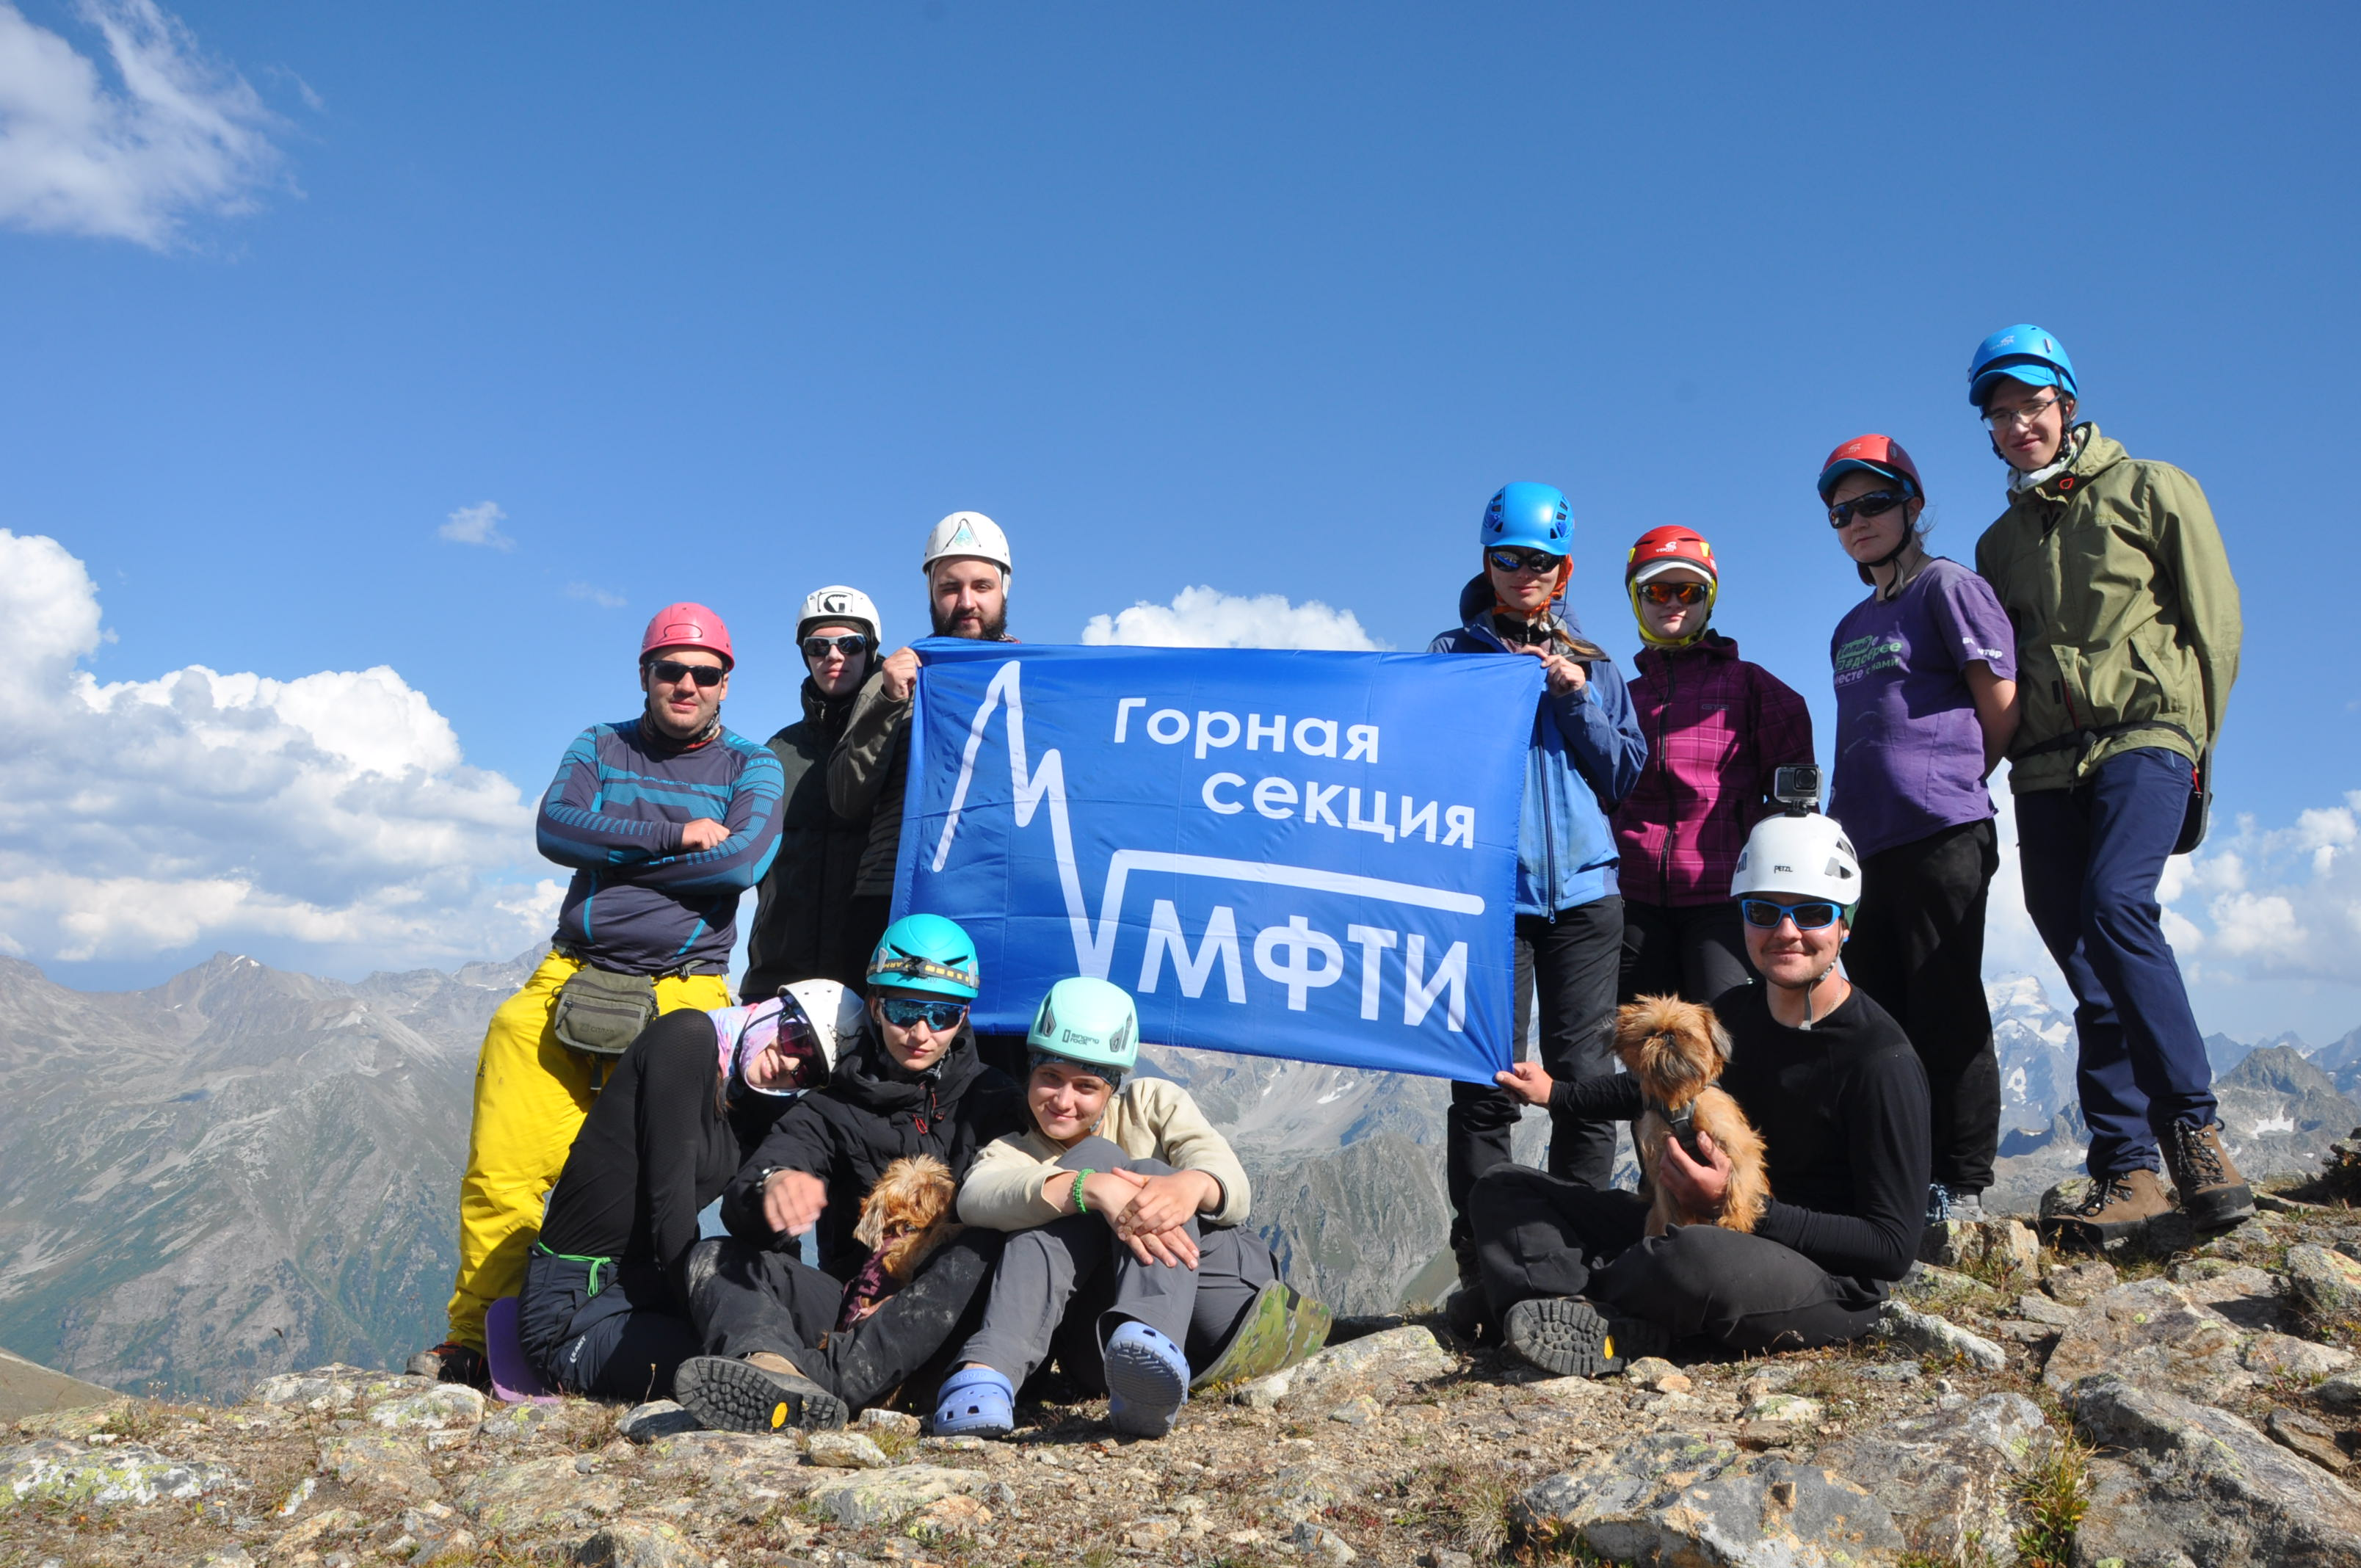
\includegraphics[width=0.7\linewidth]{../pics/DSC_0982}
	\caption{Группа на перевале, вид на д.р. Махар}
	\label{fig:DSC_0982}
\end{figure}

\begin{figure}[h!]
	\centering
	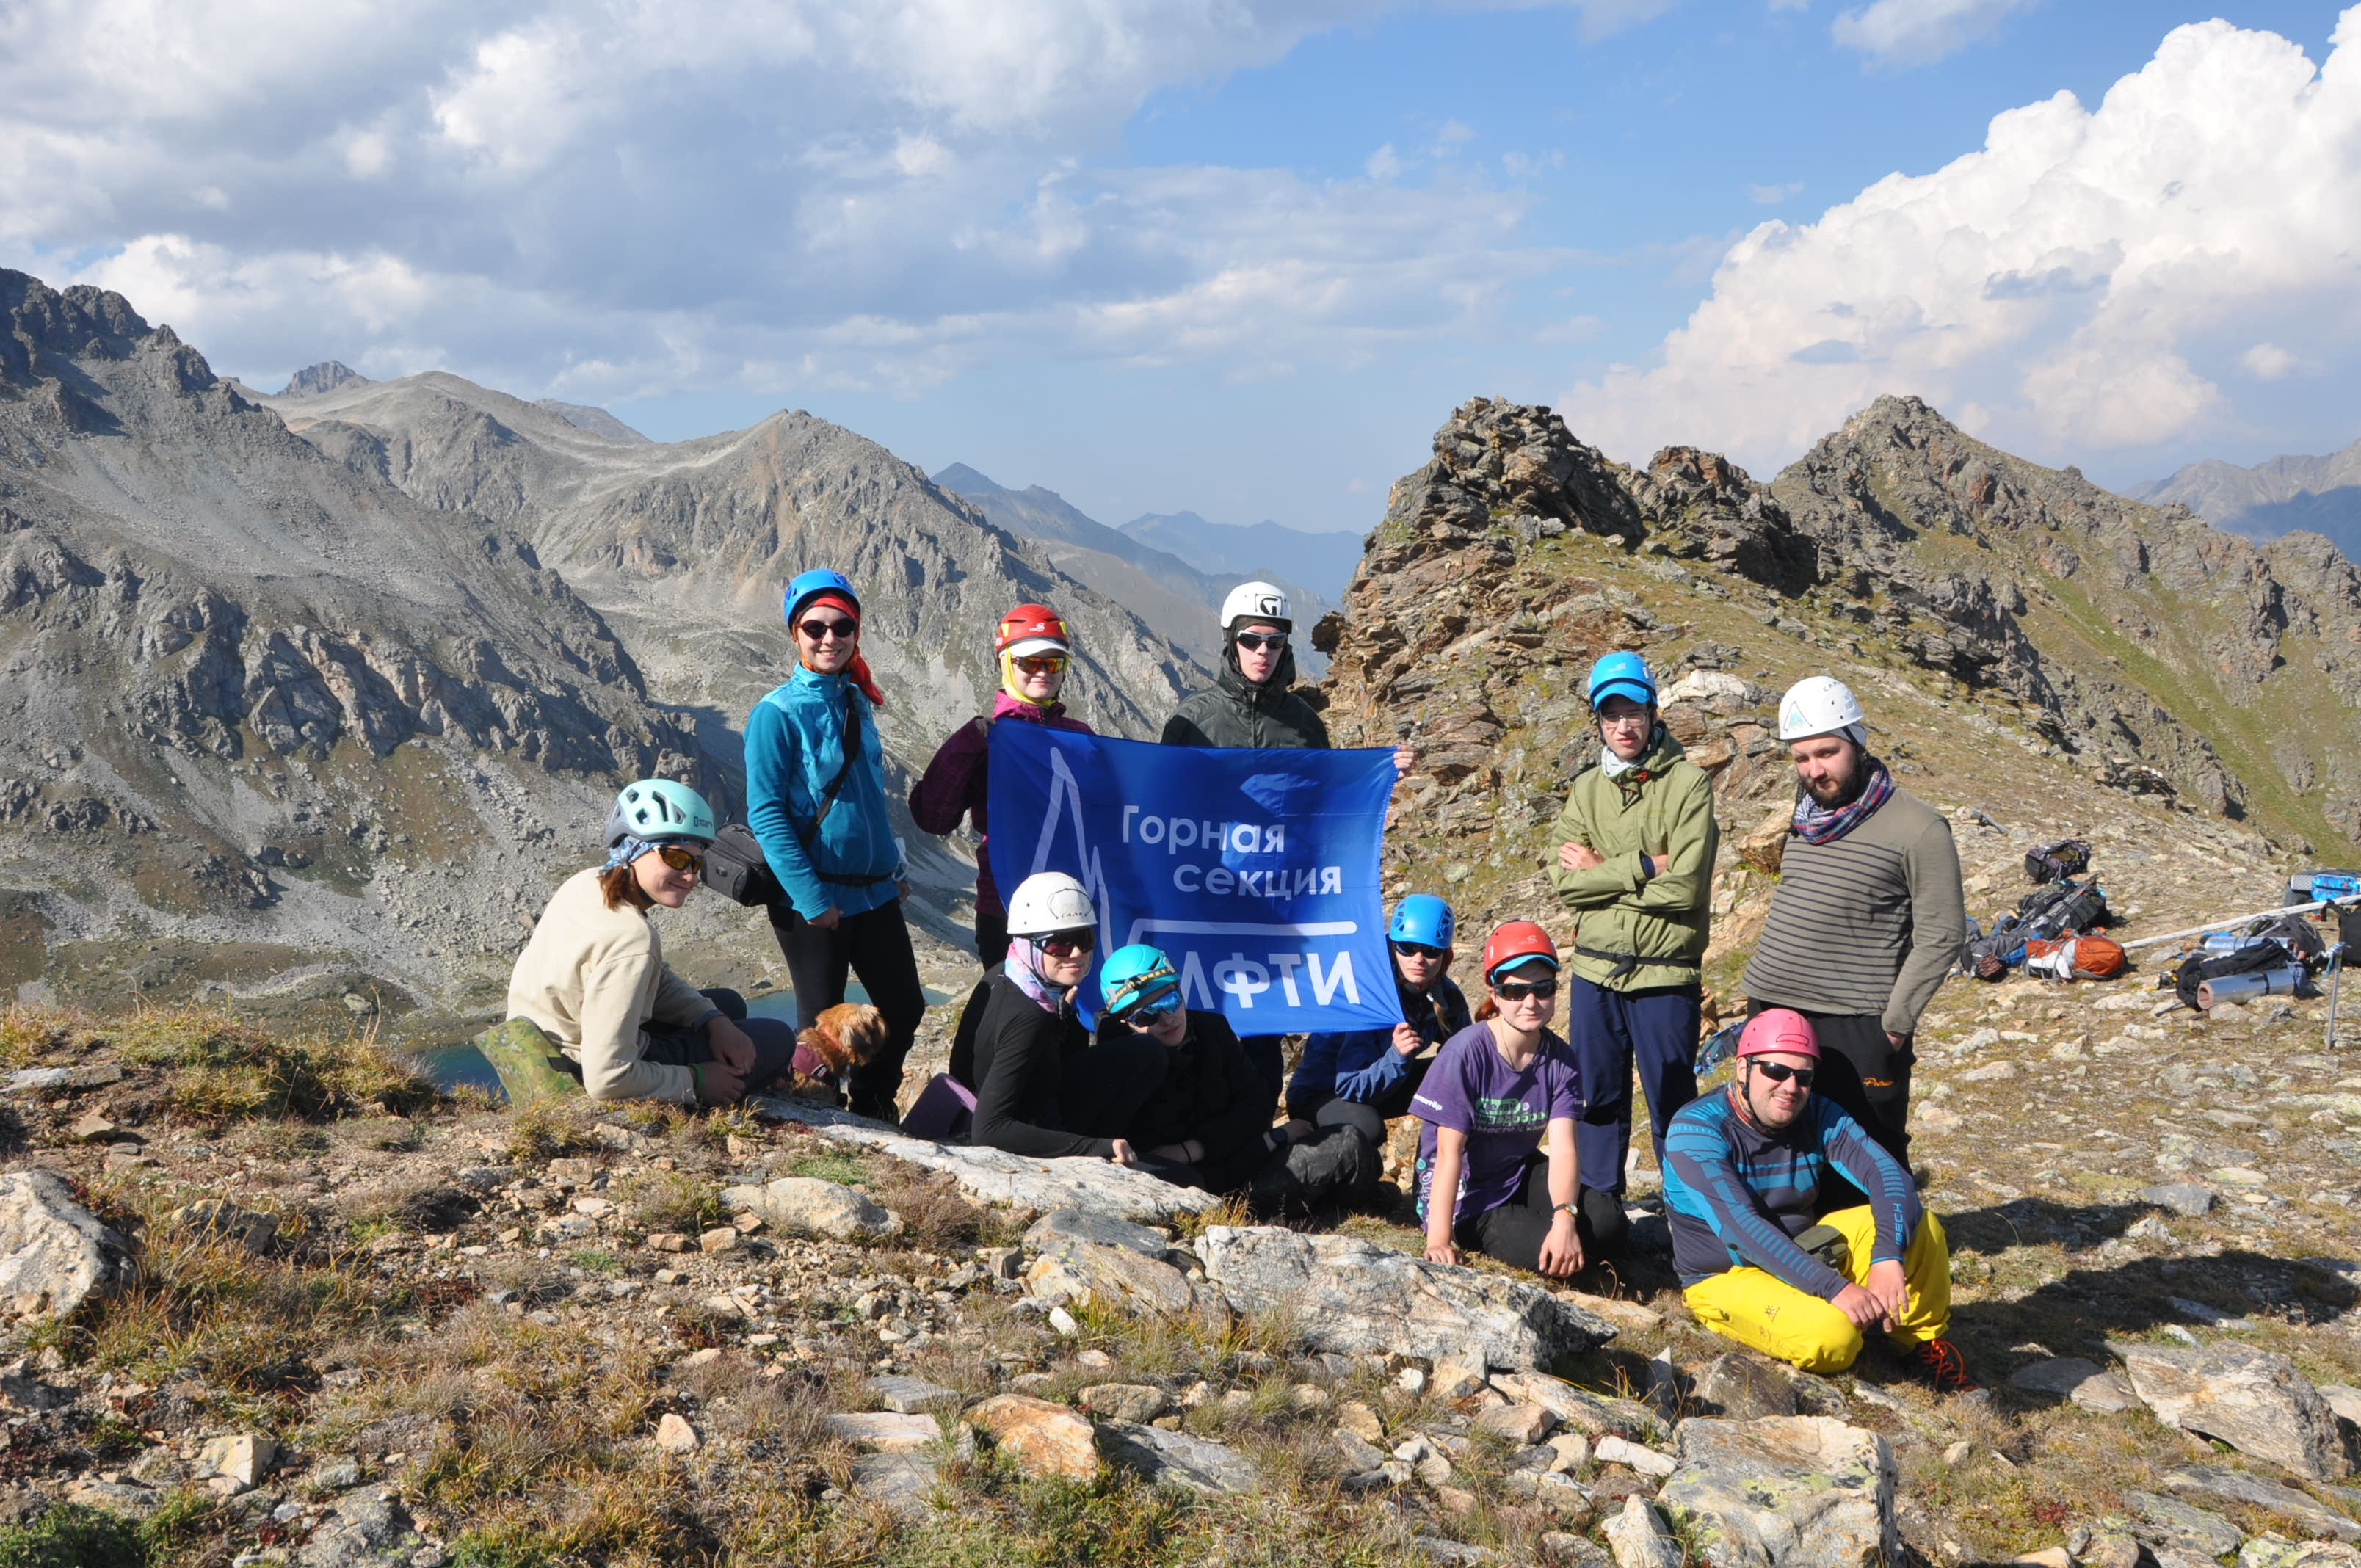
\includegraphics[width=0.7\linewidth]{../pics/DSC_0986}
	\caption{Группа на перевале, вид на оз. Уллу-Кёль}
	\label{fig:DSC_0986}
\end{figure}


В 15:48 вышли на спуск. Катя к тому моменту чувствовала себя хорошо и шла со своим рюкзаком.
Спустились к озеру по пологому травянистому склону, далее--- по гребню.

\begin{figure}[h!]
	\centering
	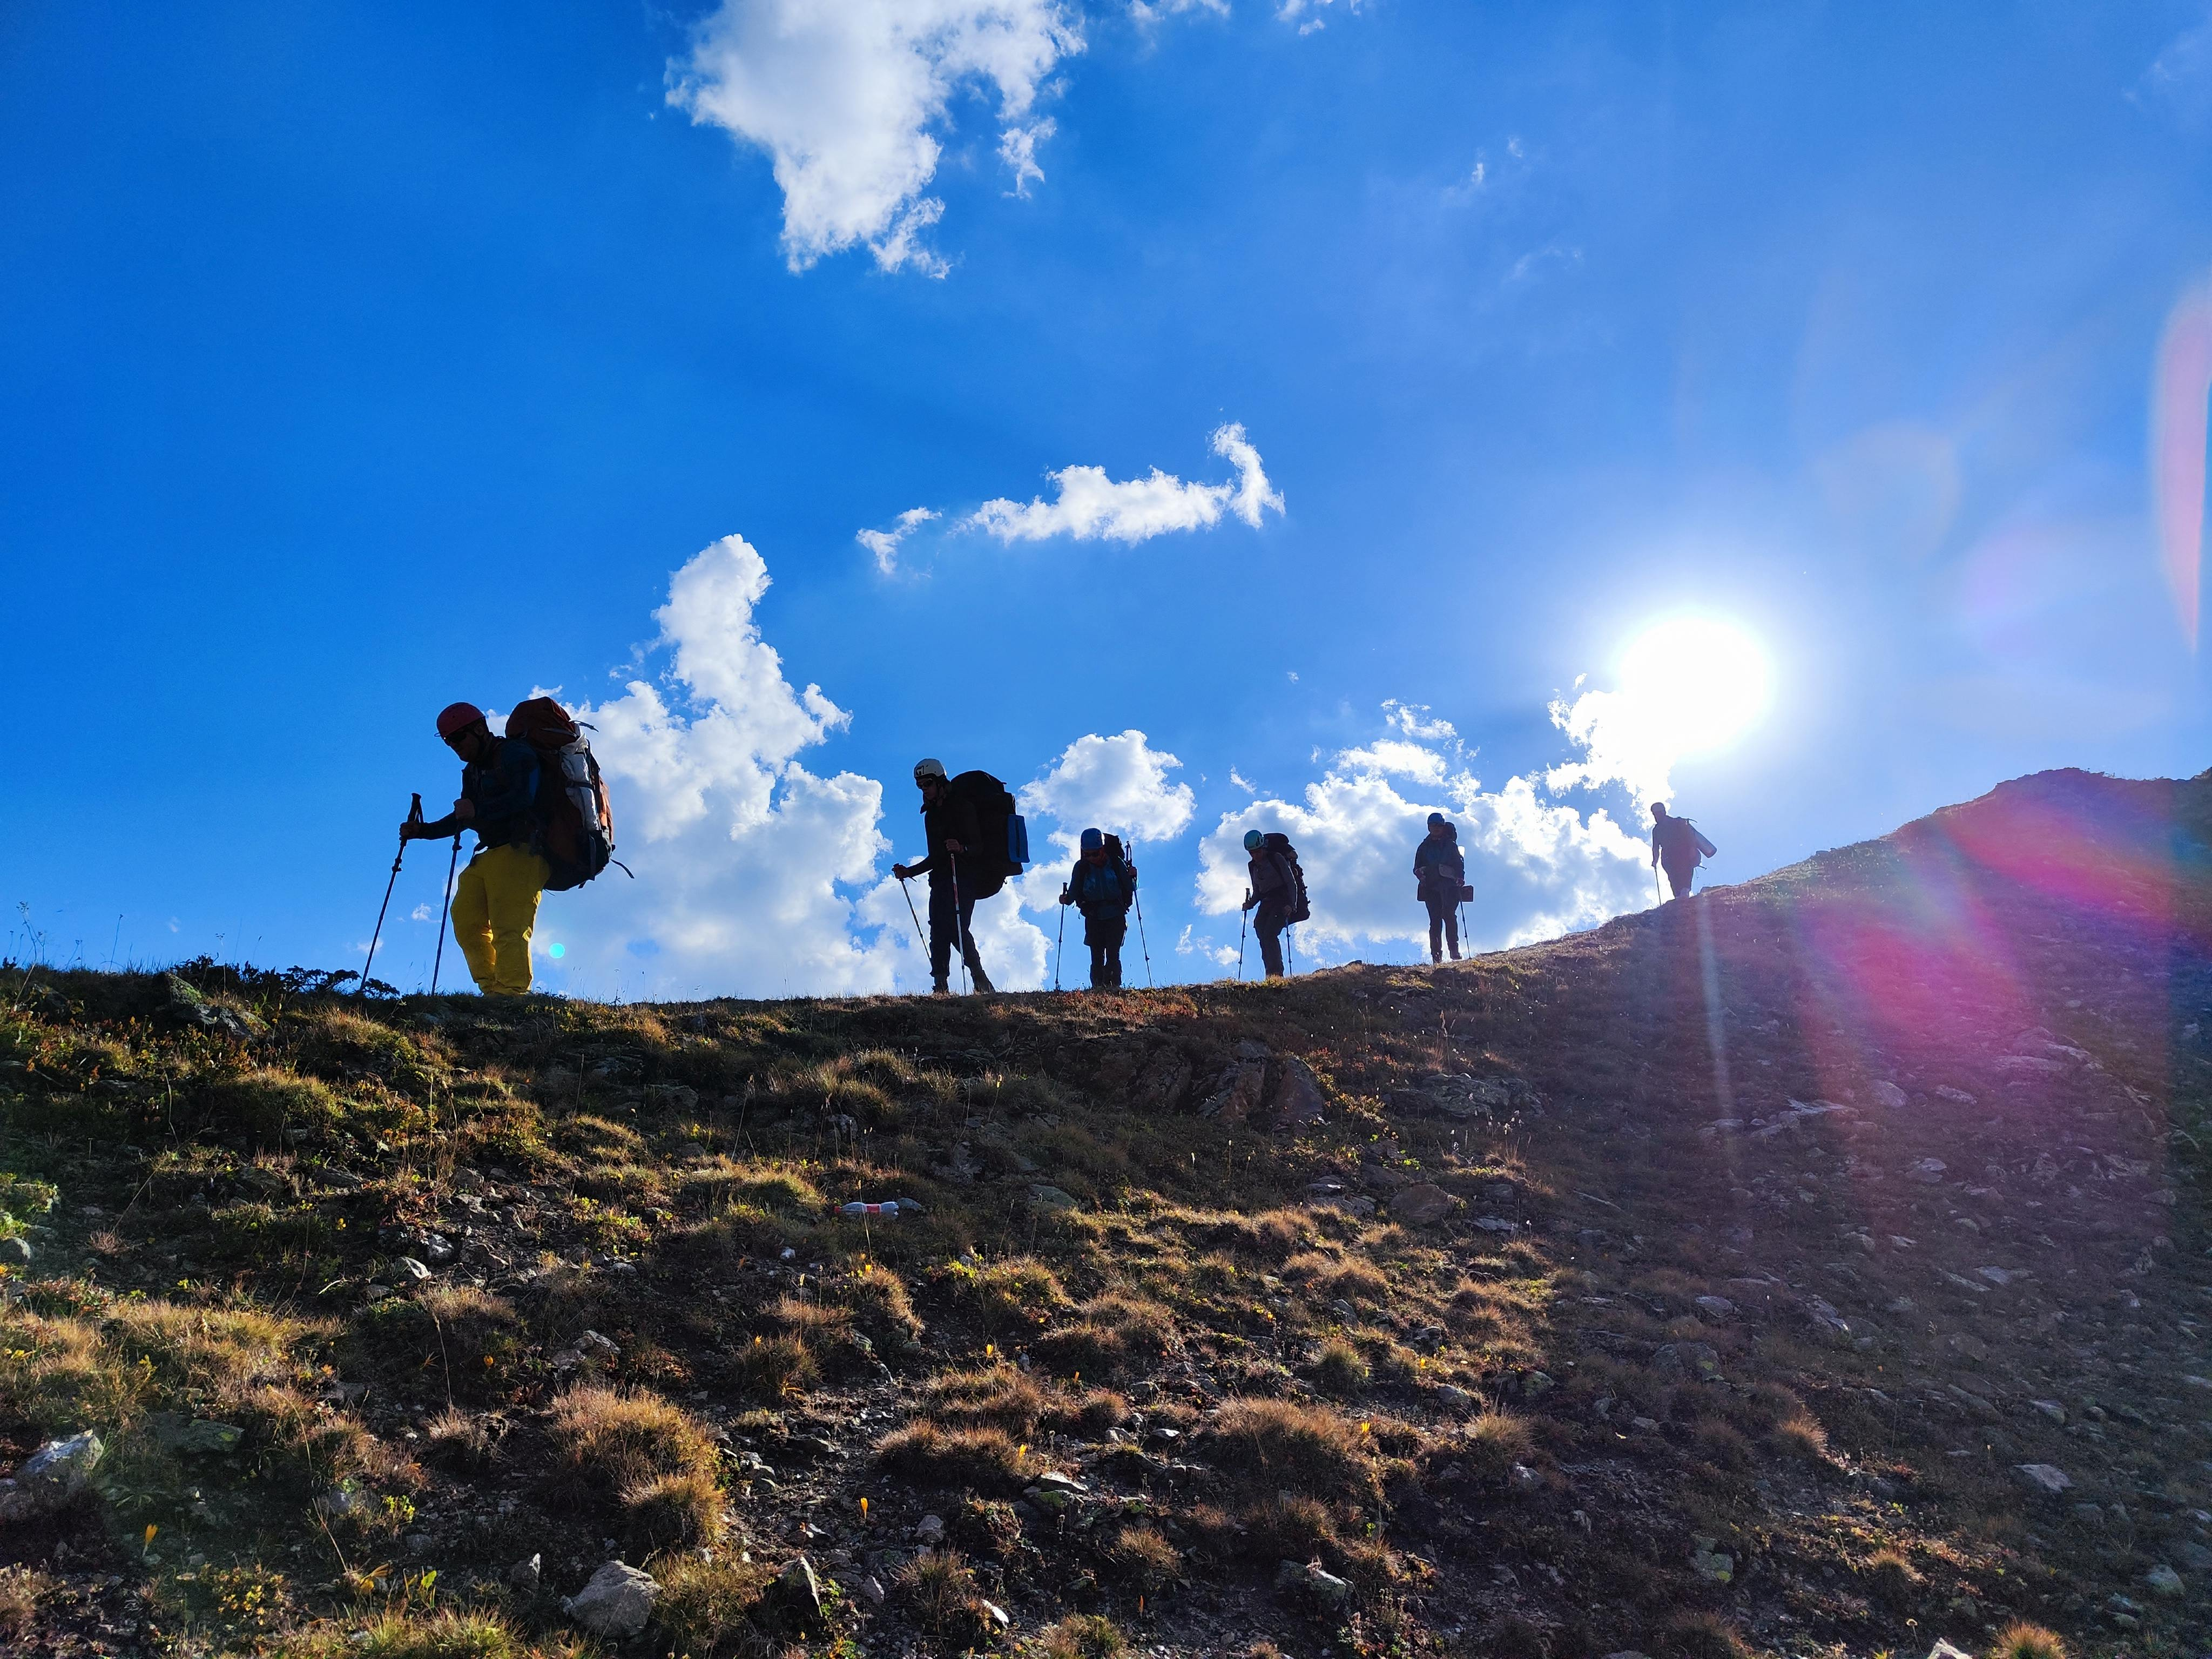
\includegraphics[width=0.7\linewidth]{../pics/IMG_20240820_164917.jpg}
	\caption{Спускаемся по гребню к озеру}
	\label{fig:IMG_20240820_164917.jpg}
\end{figure}

Пришли на озеро в 16:52, устроили обед. Было решено продолжать спуск, чтобы нагнать график: в противном случае весь следующий день был бы потрачен на заход по долинам, и подняться в д.~р. Джалпаккол мы бы тогда скорее всего не успели, что далее практически гарантированно приводило бы к потере дня. Вышли в 18:10; самой опасной на тот момент виделась ситуация, при которой группа ошибочно выходит на ступень долины, заканчивающейся крутым обрывом и водопадом. И по описаниям, и по воспоминаниям руководителя, так могло получиться, если вовремя не подсечь тропу, ведущую из зоны альпийских лугов в зону леса. Соответственно, задача была до темноты выйти к началу зоны леса, к находящемуся там кошу, и вставать этом районе на выполаживании.  (рис.~\ref{fig:IMG_20240820_184645.jpg}).

\begin{figure}[h!]
	\centering
	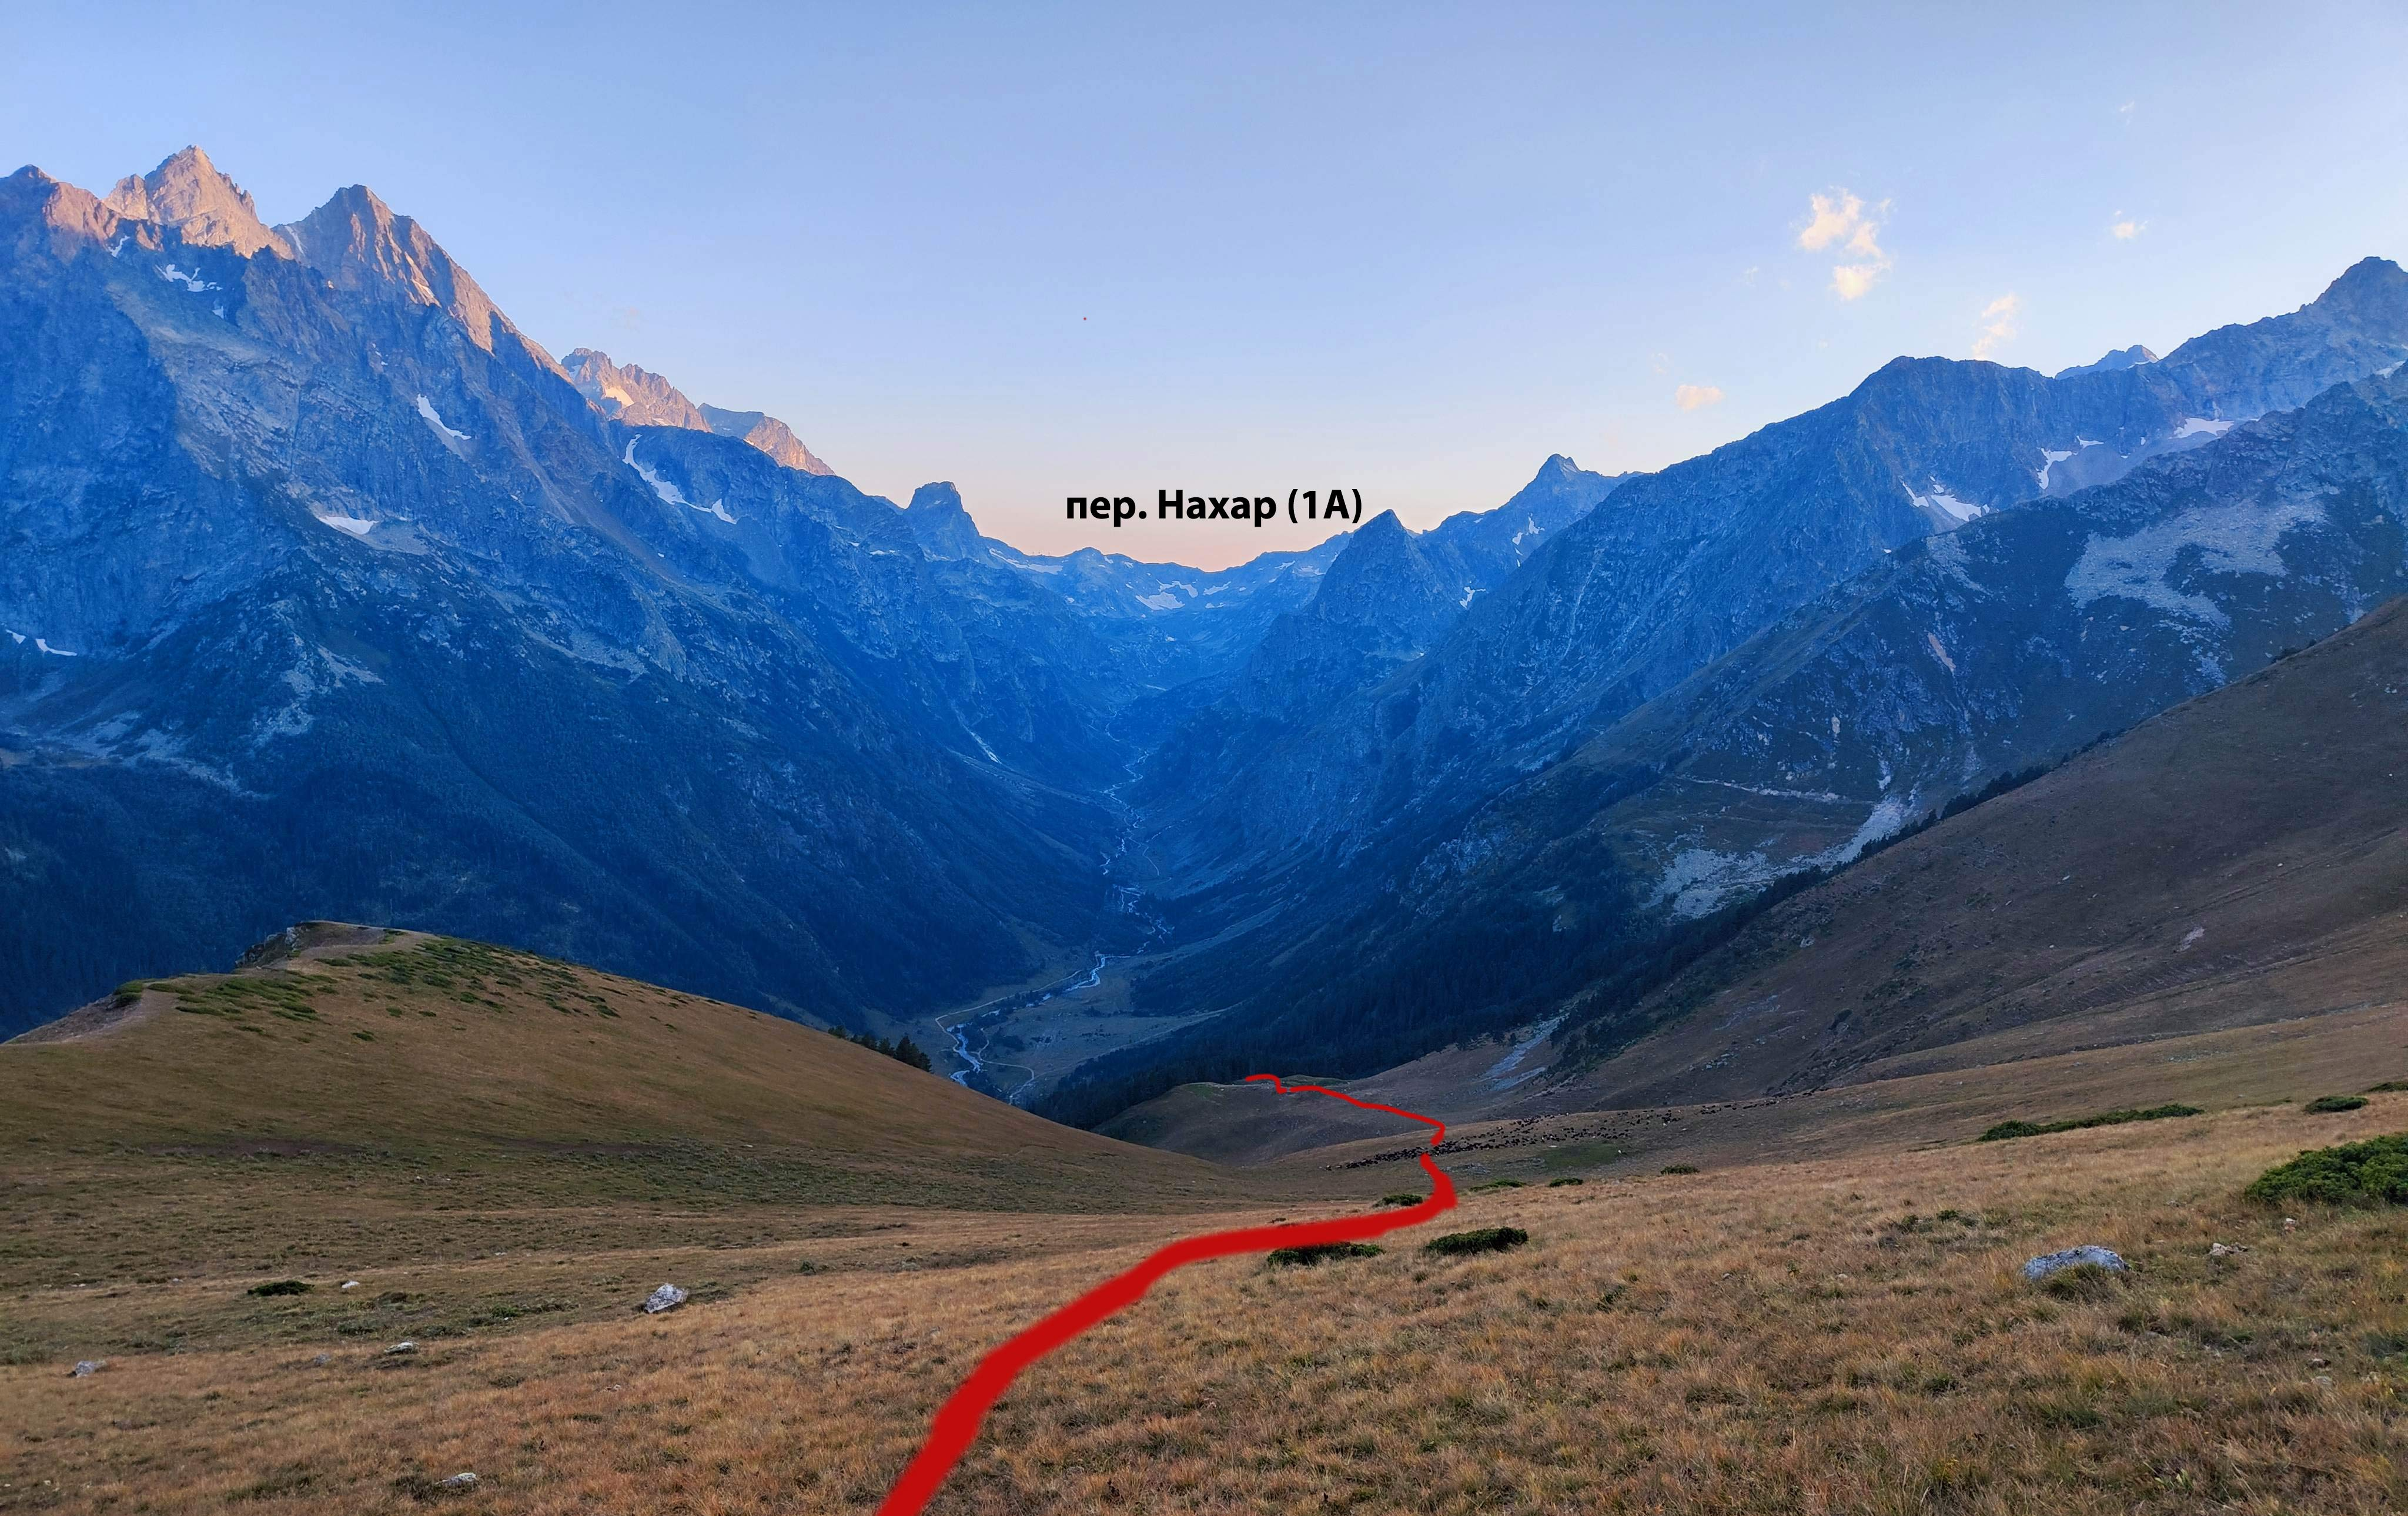
\includegraphics[width=0.7\linewidth]{../pics/IMG_20240820_184645.jpg}
	\caption{Спуск в д.р. Махар}
	\label{fig:IMG_20240820_184645.jpg}
\end{figure}

Спустились к кошу в 20:16. Уже темно, идём с фонариками, которые надели за 1 км до коша, на пастбищах. Как и группе Королёва в своё время, нам повезло встретить пастуха и узнать у него, что до долины 1.5~км по хорошей, но крутой тропе, с 500 м сброса. В группе провели голосование, в ходе которого решено было всё-таки спускаться в долину и ночёвать внизу. Тропа идёт по густому лесу, на начальном участке узкая, в момент выхода к р. Трёхозёрная становится шире. Спуск по ней действительно оказался технически несложным, но довольно крутым, и по-хорошему требовал подстраховки альпенштоком. Дополнительно мешали спуску пыль и мошки, а также, несмотря на приподнятое настроение в группе, сильно сказывалась общая усталость.

В 22:15 встали на ночёвку в д.р. Махар, координаты м.н. N43.294527\degree,~E41.956866\degree.

\clearpage 

\begin{table}[h!]
	\centering
	\begin{tabular}{|c|c|c|c|c|c|} 
		\hline 
		Этап & ЧХВ \\ 	
		\hline 
		Подъём в д.р. Кичкинакол Уллукёльский  & 02:10 \\
		Подъём по д.р. Кичкинакол Уллукёльский  & 04:23 \\
		От м/н до начала осыпного перевального взлёта & 01:33\\ 
		По перевальному взлёту до снежника & 01:22\\ 
		По снежнику до седловины (не считая срыва участника) & 00:40\\ 
		К озеру & 00:57 \\
		К кошу пастухов & 01:56 \\
		По лесу в д.р. Махар & 01:15 \\
		\hline
		\textsc{Полное время подъёма на перевал  }& 10:08\\
		\textsc{Полное время спуска с перевала }& 04:08 \\
	\textsc{	Полное время прохождения перевала }& 14:16 \\
		\hline
	\end{tabular}
	\caption{Расклад времени, пер. Уллу-Кёль Восточный}
\end{table}

\paragraph{Выводы и рекомендации:} Наш опыт подтверждает, что категория сложности перевала занижена. В малоснежный сезон снежный карниз отсутствует, однако перемещение по осыпному и снежному склонам требует определённого уроовня подготовки группы. В снежный сезон для неопытной группы провешивать перила при такой крутизне склона потребуется почти наверняка. В новичковом походе проходить Уллу-Кёль Восточный первым по счёту перевалом не рекомендуется, поскольку, хотя его прохождение и даёт возможность посмотреть на красивое озеро Уллу-Кёль, но велик риск, во-первых, излишне утомить группу, а во-вторых --- сформировать неправильное представление о характерной сложности перевалов категории 1А, а это может иметь непредсказуемые последствия. 

\clearpage
